\documentclass{article}
\usepackage[utf8]{inputenc}
\usepackage{geometry}
\usepackage{graphicx}
\usepackage{pgfplots}
\usepackage{verbatim}
\usepackage{amssymb}
\usepackage{amsmath}
\usepackage{tcolorbox} %needed
\usepackage{comment}
\usepackage{physics}
\tcbuselibrary{listingsutf8}


\geometry{a4paper, left=2cm, right=2cm, top=1cm, bottom=2cm}
\pgfplotsset{compat=1.18}

\begin{document}

\subsection*{I. Usando el metodo de exhaución, obtener:} \\
(a) El ́area de un círculo de radio r. \\
\textit{De acuerdo a la fórmula del área de un polígono regular de n lados obtenemos que:}
\begin{equation*}
    A_p = \frac{nla}{2} 
\end{equation*}
\begin{figure}[h]
    \centering
    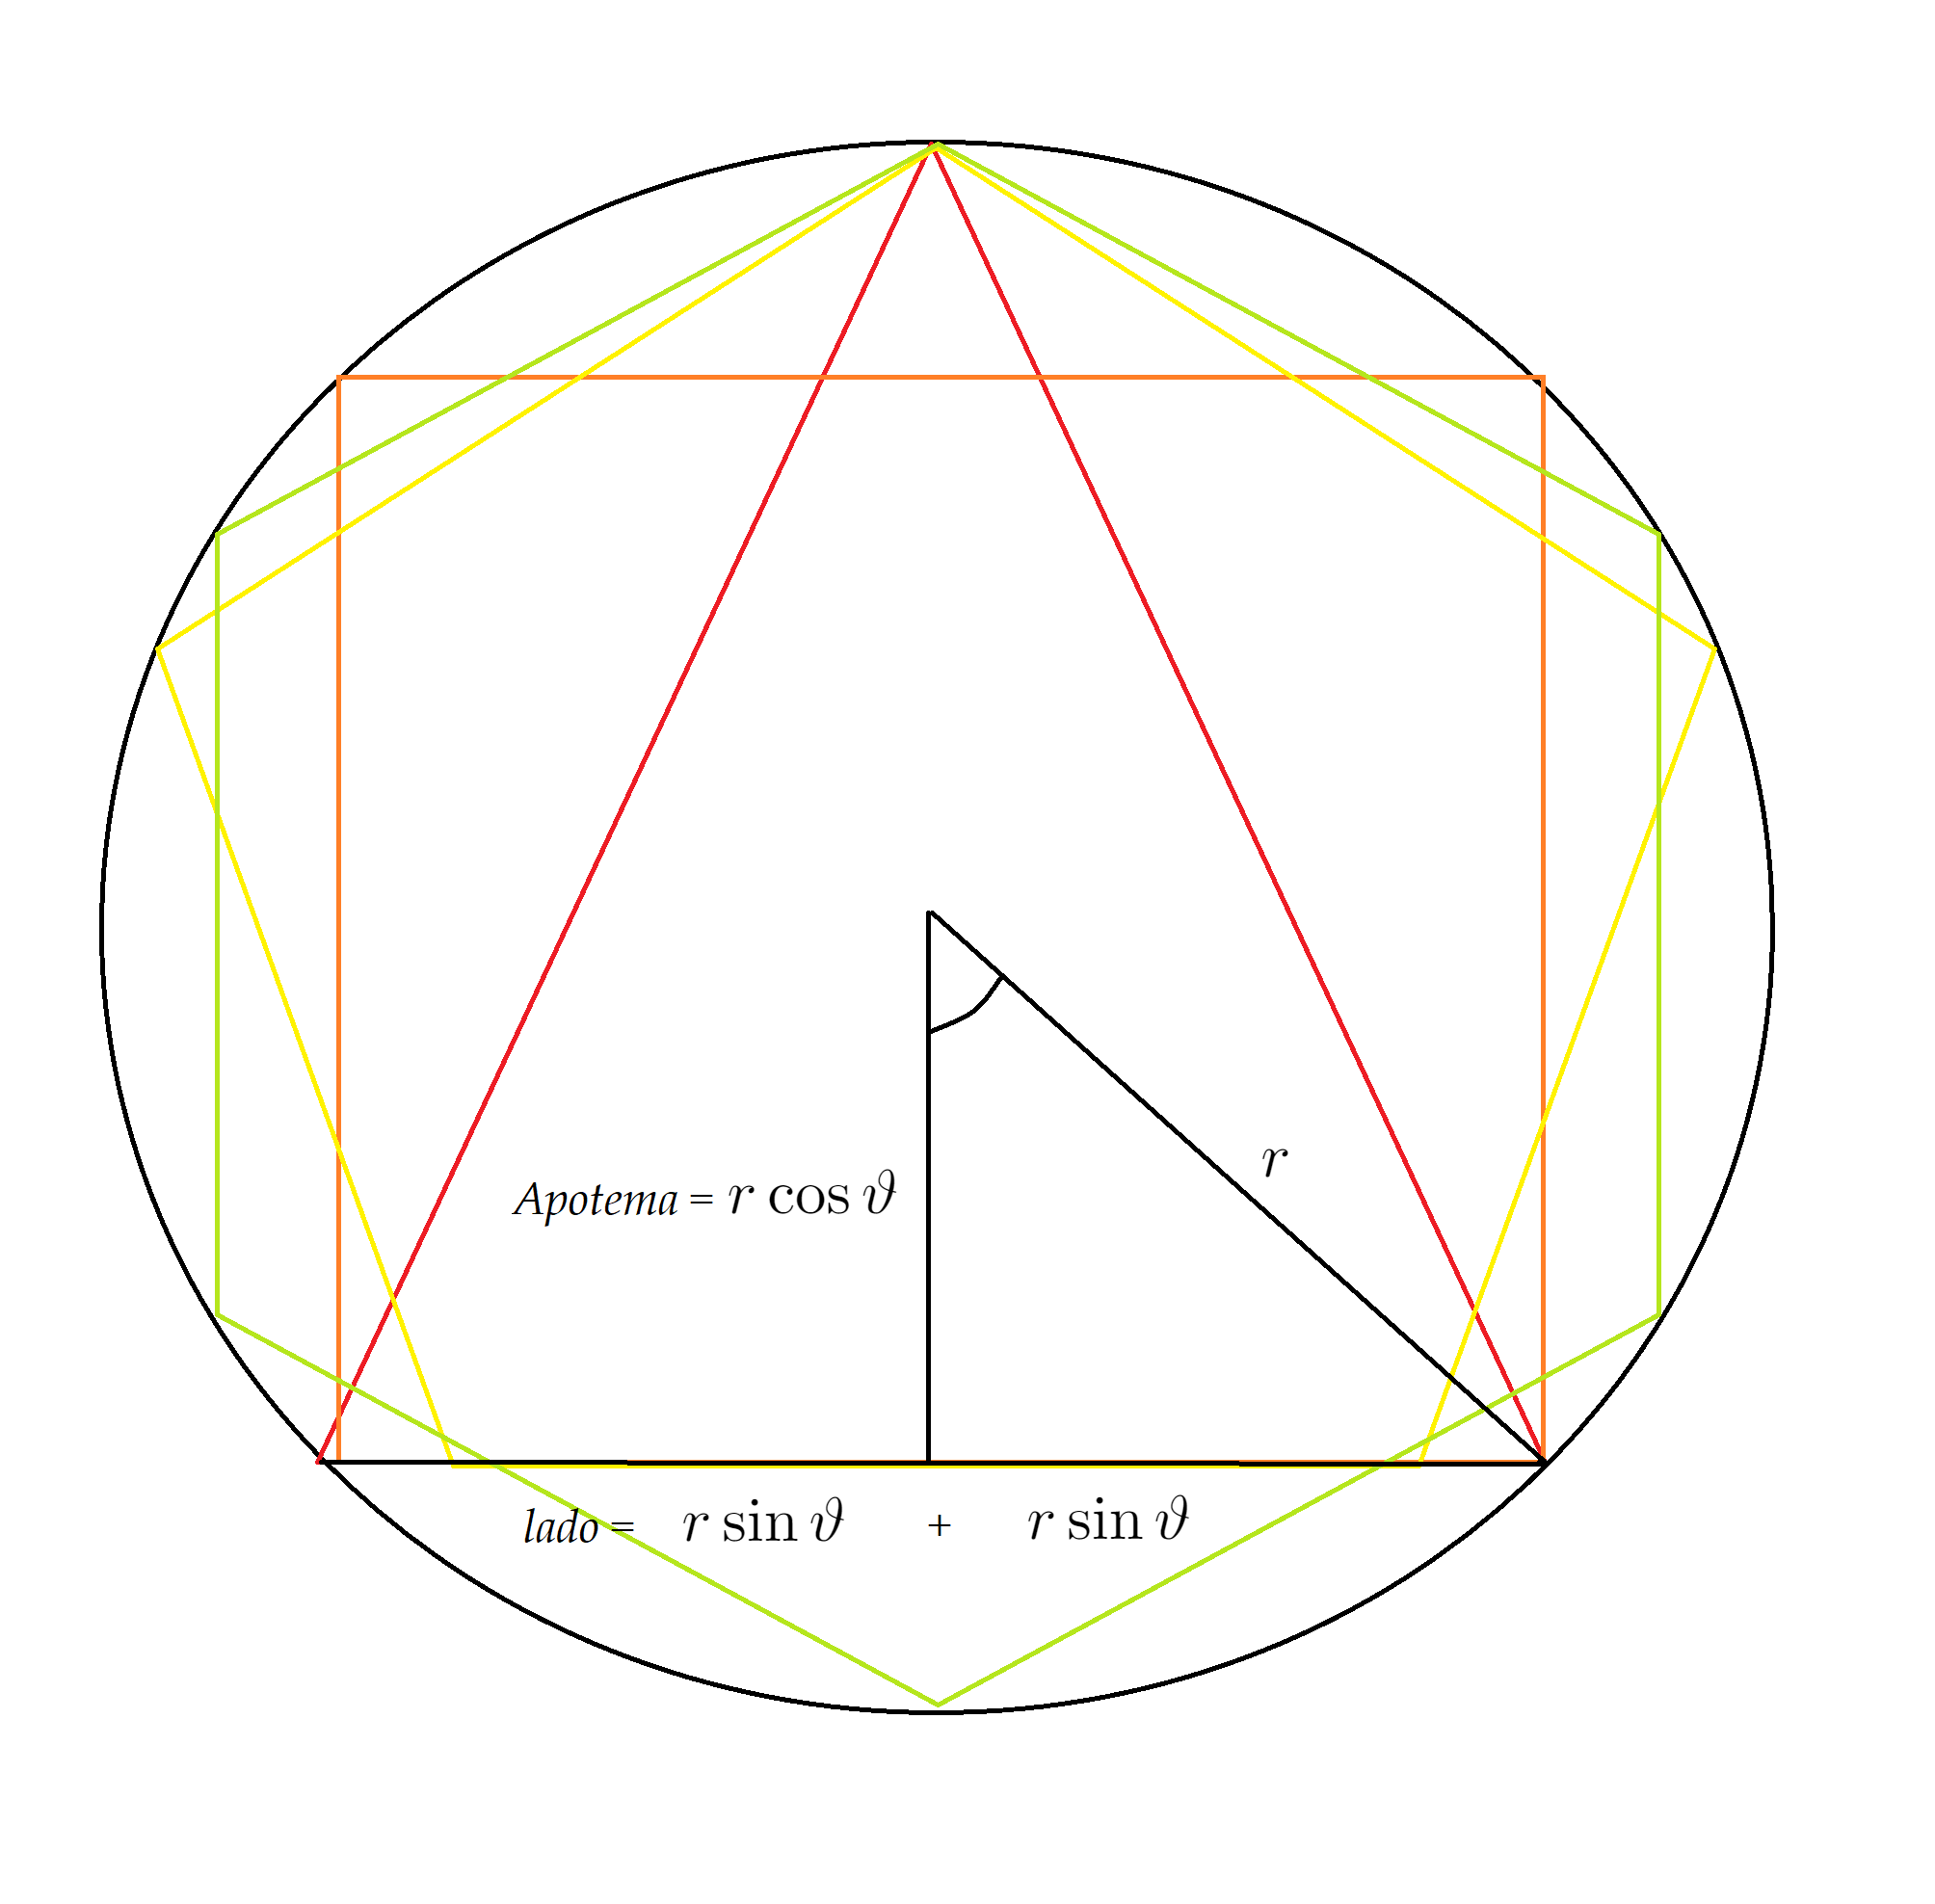
\includegraphics[width=0.45\linewidth]{circuloarquim.png}
    \caption{Construcción de nuestra área del círculo.}
    \label{fig:enter-label}
\end{figure}\\
\textit{Un polígono de n lados está constituido por n triángulos y 2n triángulos rectángulos de ángulo $\vartheta$ (siendo este ángulo el más cercano al centro del polígono), de modo que la suma de todos sus ángulos evidentemente es $2\pi$, podemos obtener el número de lados dividiendo $2\pi$ entre el ángulo de cada triángulo no rectángulo ($2\theta$). i.e. $\frac{2\pi}{2\theta} = n = \frac{\pi}{\theta}$. Además vemos de esta ecuación que cuando n tiende a infinito entonces $\theta$ tiende a cero por derecha (valores reales), nótese que esto es lo ideal pues en un polígono por construcción no podemos tener ángulos negativos.}
$$ A_p = \frac{nla}{2} = \frac{2}{2} \cdot n \cdot r\sin \vartheta \cdot r\cos \vartheta = \frac{\pi}{\theta} \cdot r\sin \vartheta \cdot r\cos \vartheta = [\pi r^2]\left[\frac{\sin \theta}{\theta}\right][\cos \theta]$$
\textit{Ahora simplemente vemos qué valor obtiene este polígono al aplicar límite.}
\begin{equation*}
    \lim_{\theta \rightarrow 0^+} \left([\pi r^2]\left[\frac{\sin \theta}{\theta}\right][\cos \theta]\right) = [\pi r^2] \cdot \lim_{\theta \rightarrow 0^+} \left(\left[\frac{\sin \theta}{\theta}\right][\cos \theta]\right) = [\pi r^2 ] \cdot \lim_{\theta \rightarrow 0^+} \left[\frac{\sin \theta}{\theta}\right] = [\pi r^2 ] \cdot \lim_{\theta \rightarrow 0^+} \left[\frac{\dv{\sin \theta}{x}}{\dv{\theta}{x}}\right] = \pi r^2
\end{equation*}\\
\textit{Dada la idea, haremos una construcción demasiado similar acotando por polígonos en el exterior de la circunferencia, visualmente en Figure II y considerando que $\alpha$ es el ángulo de cada triángulo compuesto de dos triángulos rectángulo nótese que $\alpha = \frac{2\pi}{n} \Rightarrow \frac{\alpha}{2} = \frac{\pi}{n}$, la altura del polígono en este caso es determinada por el radio y obsérvese atentamente en los triángulos rectángulos formados (vease la división de color rojo), tenemos que $\tan \frac{\alpha}{2} = \tan \frac{\pi}{n} = \frac{x/2}{r} \Rightarrow \frac{x}{2} = r \tan \frac{\pi}{n}$}.\\
\begin{figure}[h]
    \centering
    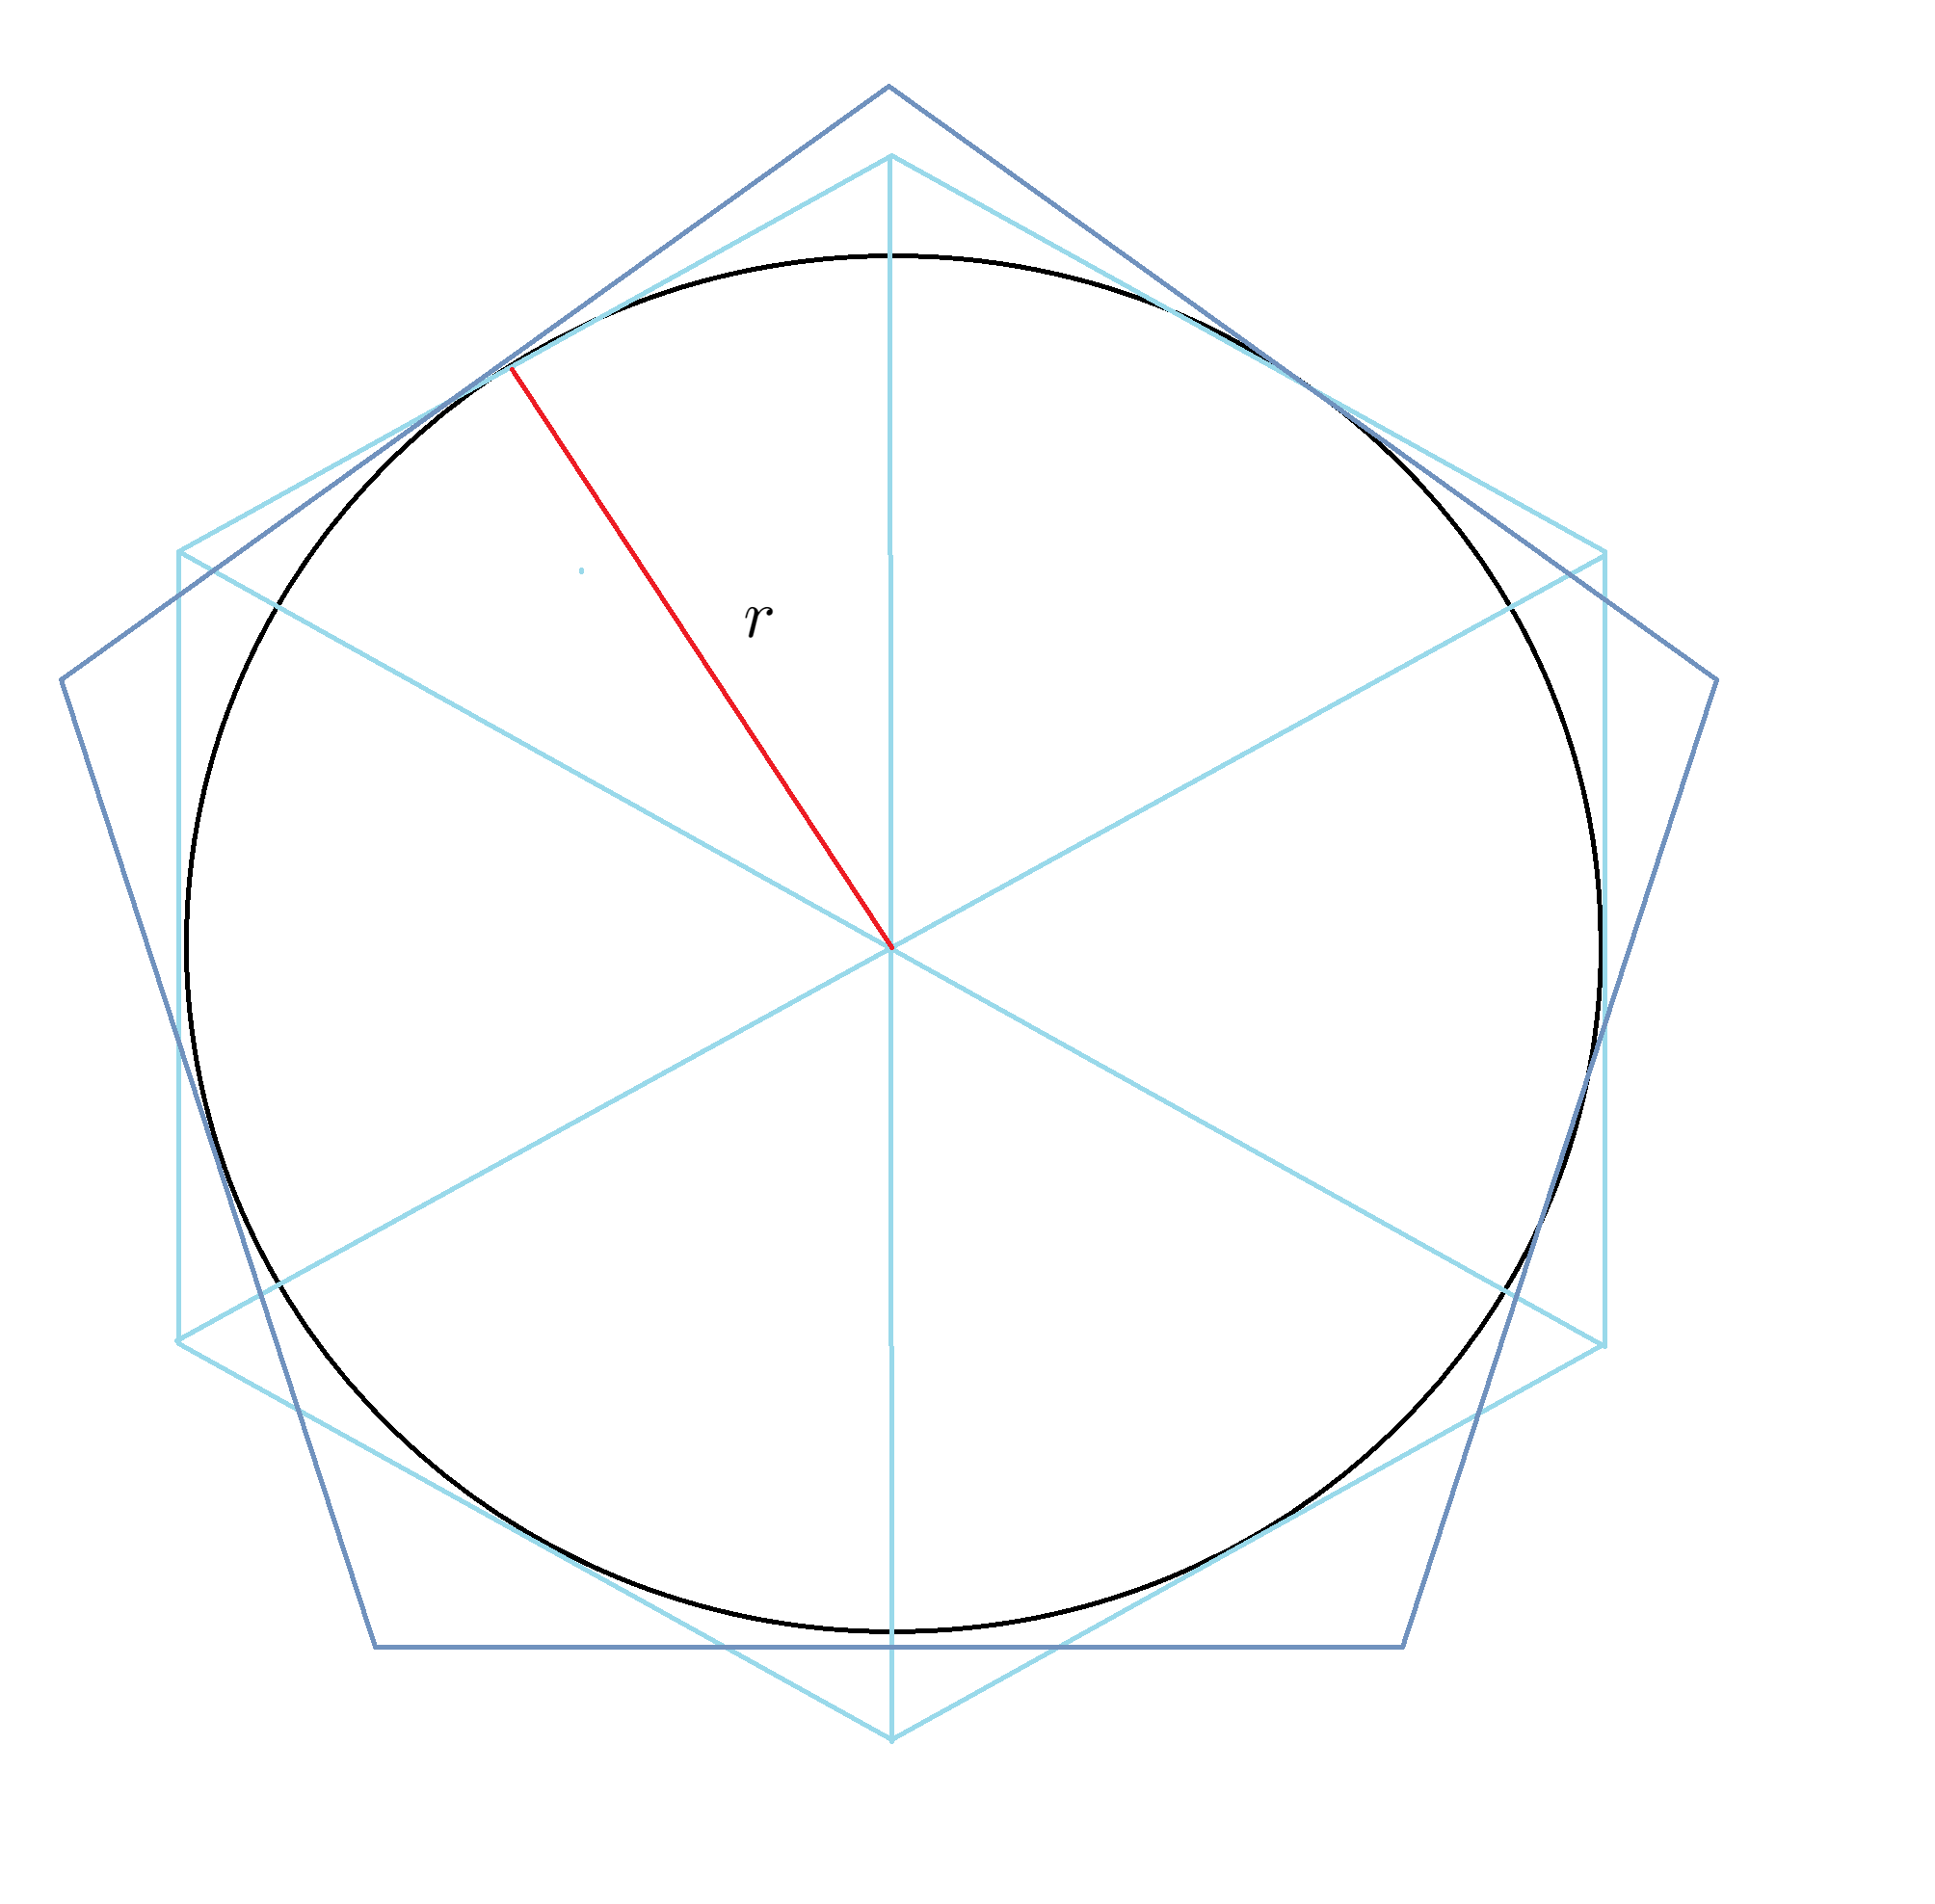
\includegraphics[width=0.45\linewidth]{nosecirculo.png}
    \caption{Construcción círculo que acota superiormente.}
    \label{fig:enter-label}
\end{figure}
\textit{El área del polígono se determina similarmente por:}
\begin{align*}
    A_p &= \frac{nla}{2} \\
    &= \frac{2nr^2 \tan \frac{\pi}{n}}{2} \\
    &= nr^2 \tan \frac{\pi}{n} \\
    &= \pi r^2 \frac{\tan \frac{\pi}{n}}{\frac{\pi}{n}}
\end{align*}
\textit{Aplicamos el límite cuando el número de lados tiende a infinito a esta función.}\\
\begin{align*}
    \lim_{n \rightarrow \infty} \pi r^2 \frac{\tan \frac{\pi}{n}}{\frac{\pi}{n}} &= \pi r^2  \lim_{n \rightarrow \infty} \frac{\tan \frac{\pi}{n}}{\frac{\pi}{n}} \\
    &= \pi r^2  \lim_{n \rightarrow \infty} \frac{\sin \frac{\pi}{n}}{\frac{\pi}{n}} \cdot \sec \frac{\pi}{n} \\
    &= \pi r^2
\end{align*}
\textit{Obsérvese que nuestra primera función está compuesta de una sucesión creciente de polígonos que están en el interior del círculo y a lo más en cada vértice toca la frontera de este, mientras que nuestra segunda función es una sucesión decreciente de polígonos quienes convergen a la frontera del círculo y cada polígono toca a lo más la parte de cada lado que conecta con el apotema, como el área del círculo se queda compactada por estas dos sucesiones obtenemos que.}
\begin{align*}
    A_{inf.c} \leq &A \leq A_{sup.c} \\
    \pi r^2 \leq &A \leq \pi r^2
\end{align*}
$\therefore$ \textit{Por compactación que indujo la tricotomía, el área de nuestro círculo es $\pi r^2.$}

(b) El volumen de un cono circular recto de altura $h$ y radio $r$.\\
\textit{Nuestra construcción del área del cono es haciendo iteraciones de cilindros constituidos de altura $h_i$ y radio $h_i$ variante dependiente de cada iteración de la suma véase en Figure III. Por teorema de tales tenemos la relación $\frac{r}{h} = \frac{r_i}{h_i}$. Obtenemos los siguientes datos para $h_i$ y $r_i$.}
$$ h_i = \frac{h}{n}, \quad r_i = \frac{r}{h} \cdot \frac{h}{n} \cdot i = \frac{ri}{h}, \quad V_{cilindro} = bh = \pi r_i^2 h_i $$
\newpage
\begin{figure}[h]
    \centering
    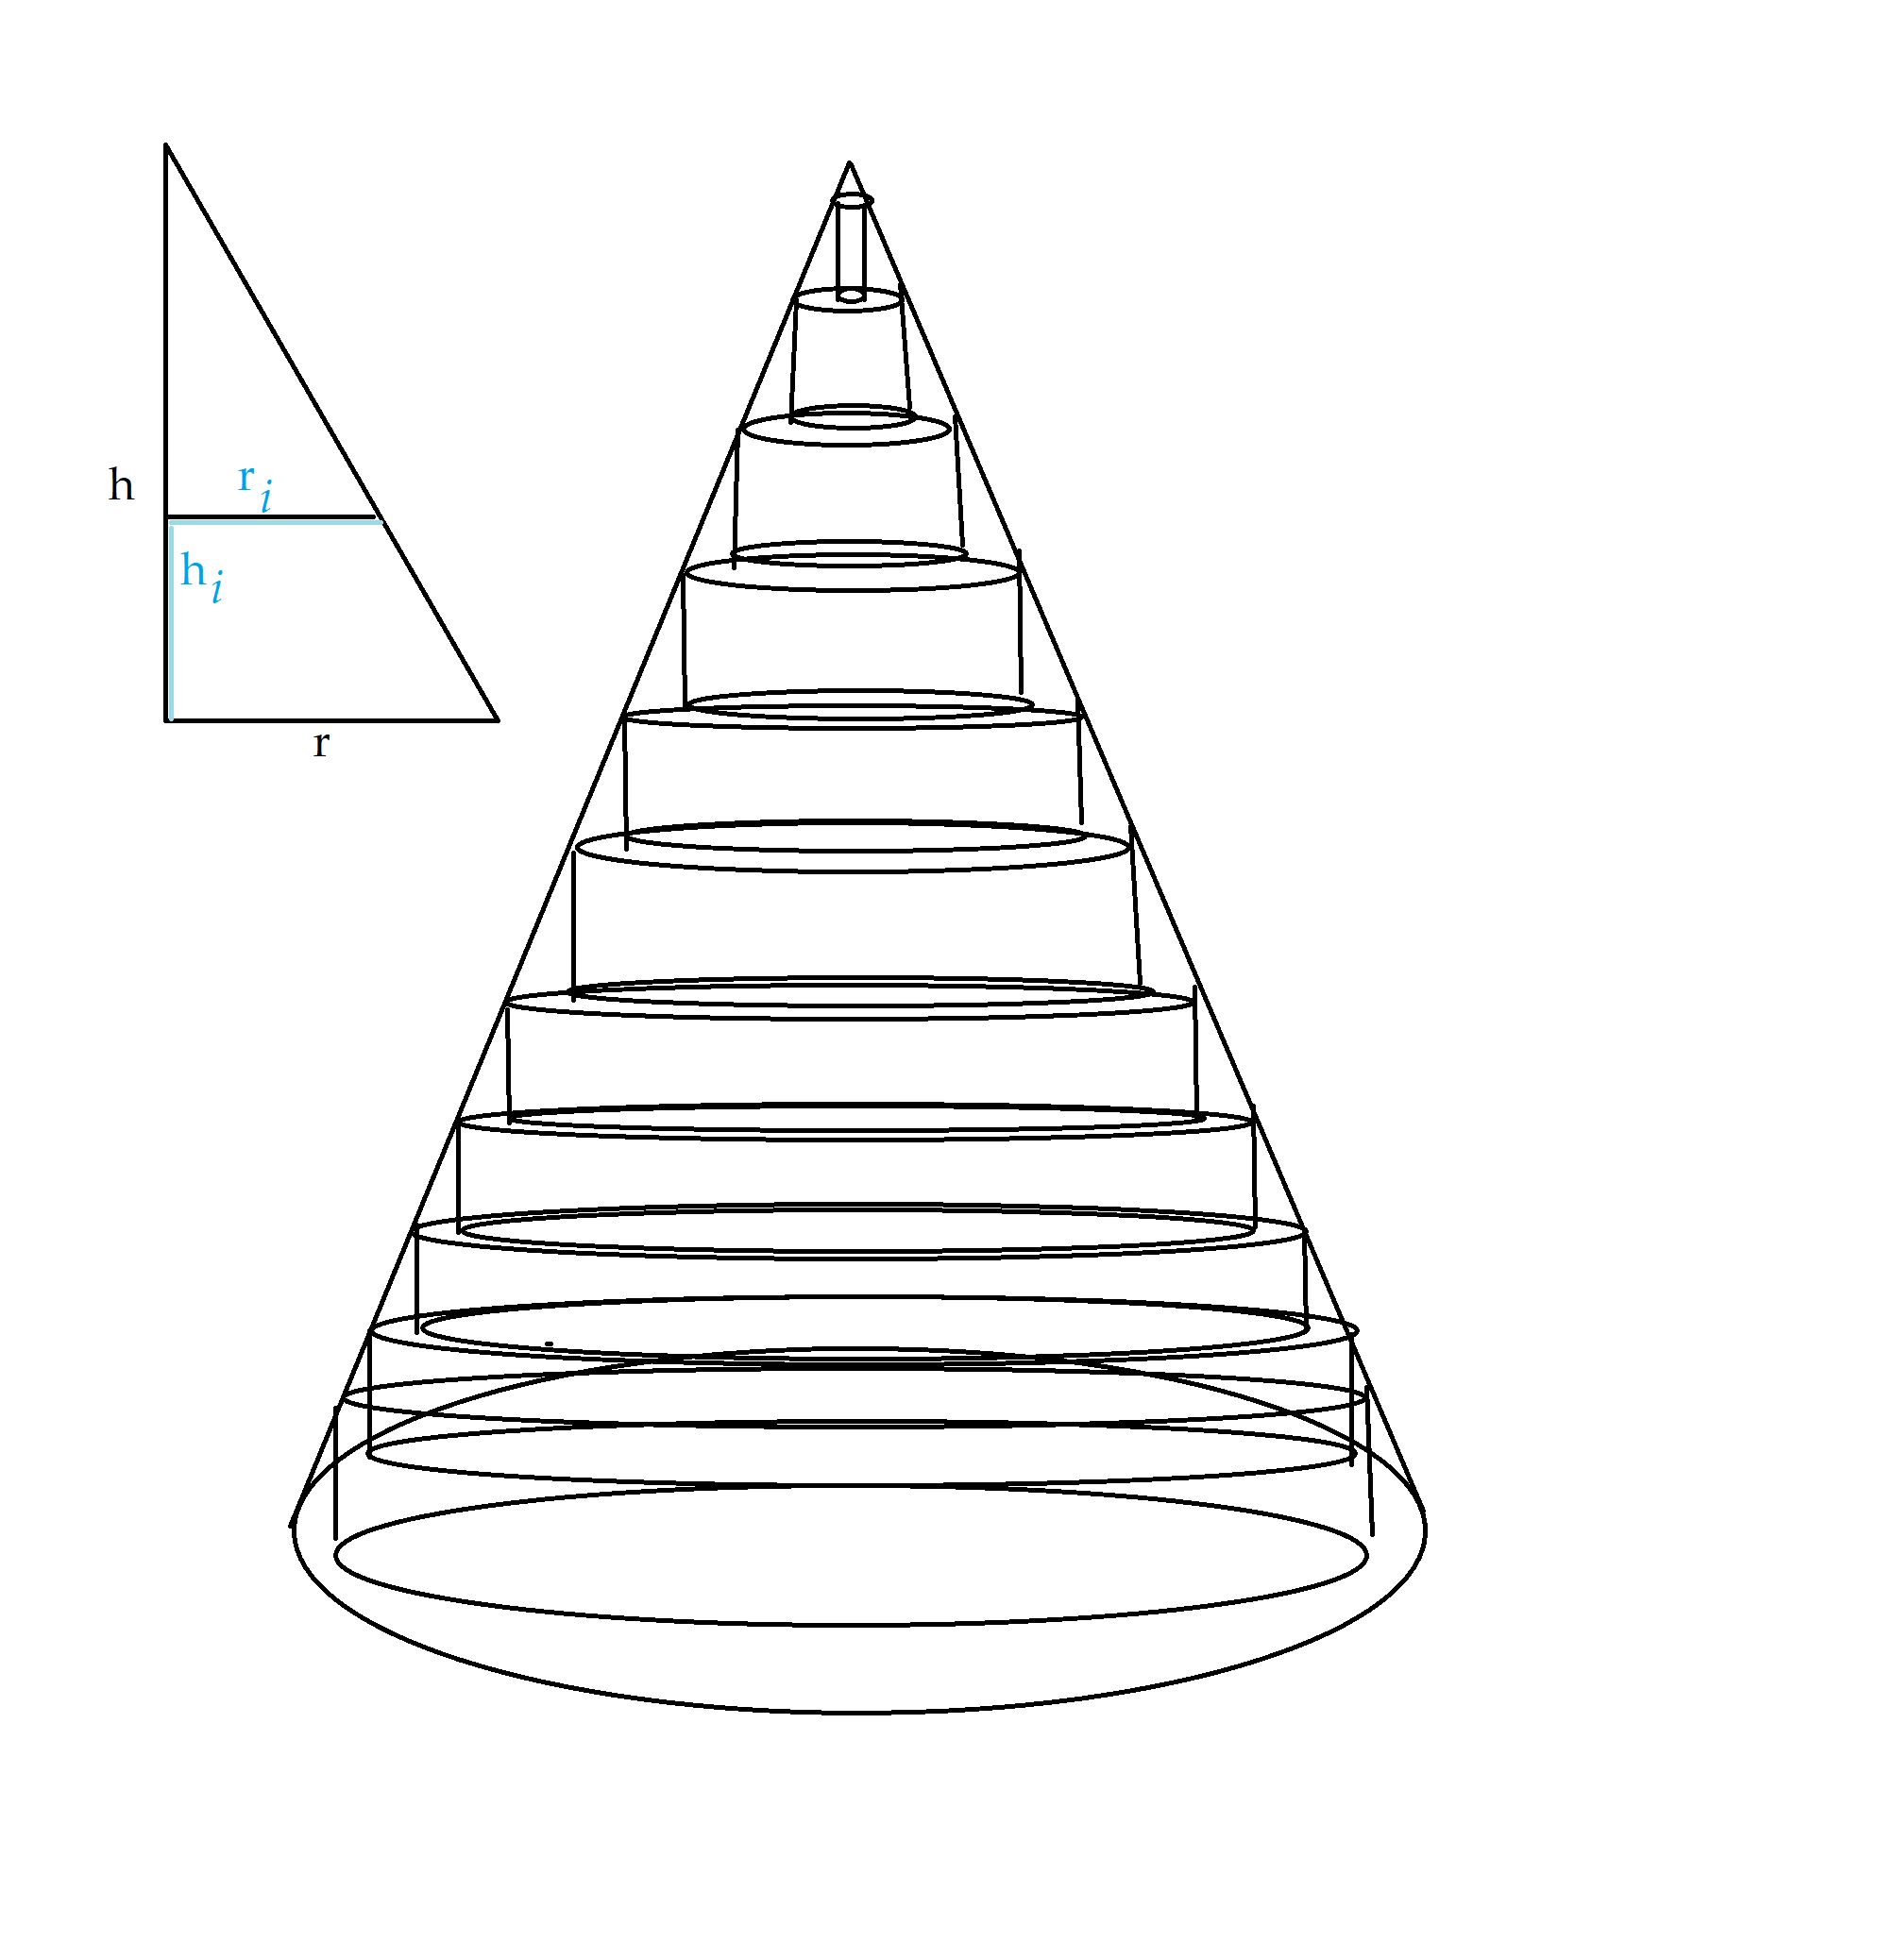
\includegraphics[width=0.45\linewidth]{conitoconcilindritos.png}
    \caption{Construcción del volumen del cono.}
    \label{fig:enter-label}
\end{figure}
\begin{align*}
    \textit{Aproximación del volumen del cono} &= \sum_{i=1}^n V_{cilindro (i)}\\
    &= \sum_{i=1}^n \pi r_i^2 h_i \\
    &= \sum_{i=1}^n \pi \frac{r^2i^2}{n^2} \frac{h}{n} \\
    &= \sum_{i=1}^n \frac{\pi r^2 h}{n^3}i^2 = \left[ \frac{\pi r^2 h}{n^3} \right] \left[ \frac{n(n+1)(2n+1)}{6} \right] = \left[ \frac{\pi r^2 h}{n^3} \right] \left[ \frac{2n^3 + 3n^2 + n}{6} \right]
\end{align*}
\textit{Dada esta ecuación final vemos qué sucede cuando el número de particiones en cilindros tiende a infinito, nótese que en este inciso como el anterior $n$ deja de tener caracter natural y pasa a ser un real para obtener valores exactos.}
\begin{align*}
    \lim_{n \rightarrow \infty} \left[ \frac{\pi r^2 h}{n^3} \right] \left[ \frac{2n^3 + 3n^2 + n}{6} \right] &= [\pi r^2 h] \cdot \left[ \lim_{n \rightarrow \infty} \frac{2n^3+3n^2+n}{6n^3} \right] \\
    &= [\pi r^2 h] \cdot \left[ \lim_{n \rightarrow \infty} \frac{\dv{[2n^3+3n^2+n]}{n}}{\dv{[6n^3]}{n}} \right] \\
    &= \frac{2\pi r^2 h}{6} \\
    &= \frac{\pi r^2 h}{3}
\end{align*}


\end{document}